\section{Scope and status of the principal results}
\label{sec:status-map}

The results form a dependency structure rather than a single derivation.
For each link, the manuscript identifies the assumption being used, the
statement proved in its place, and the model or observable that tests the
statement:
\begin{equation}
 \boxed{\begin{gathered}
 \text{stated assumption}
 \ \AssumptionArrow\
 \text{new theorem or controlled mechanism}\\[-1mm]
 \AssumptionArrow\
 \text{explicit model or observable}
 \end{gathered}}
 \label{eq:closed-loop-rule}
\end{equation}
An assumption is considered removed only when it is not replaced by an
equivalent calibration, projection, or geometric input.  This convention is
used throughout to separate operator-algebraic results from conditional
matter and cosmological extensions.

\subsection{Status conventions}

Every major statement below carries one of five statuses.
\begin{description}[leftmargin=3.6cm,style=nextline]
\item[\StatusAbstract.]
The conclusion follows from the stated operator-algebraic hypotheses and is
not tied to a finite numerical example.
\item[\StatusModel.]
The statement is exact for a specified finite-range channel or Lindbladian.
It is evidence that the relevant structure is dynamically realizable, not a
universality theorem for all quantum causal processes.
\item[\StatusNumerical.]
Part of the conclusion is a deterministic finite-size calculation,
finite-shot simulation, imported asymptotic coefficient, or model-specific
inverse theorem.  The data and the analytic components are identified
separately.
\item[\StatusConditional.]
The implication is mathematically valid only after an external continuum,
state, geometric, or field-theoretic identification is supplied.
\item[\StatusOpen.]
The item is a target mechanism or phenomenological branch.  It is not used as
support for any earlier stage of the foundational chain.
\end{description}

\begin{landscape}
\begin{figure}[p]
 \centering
 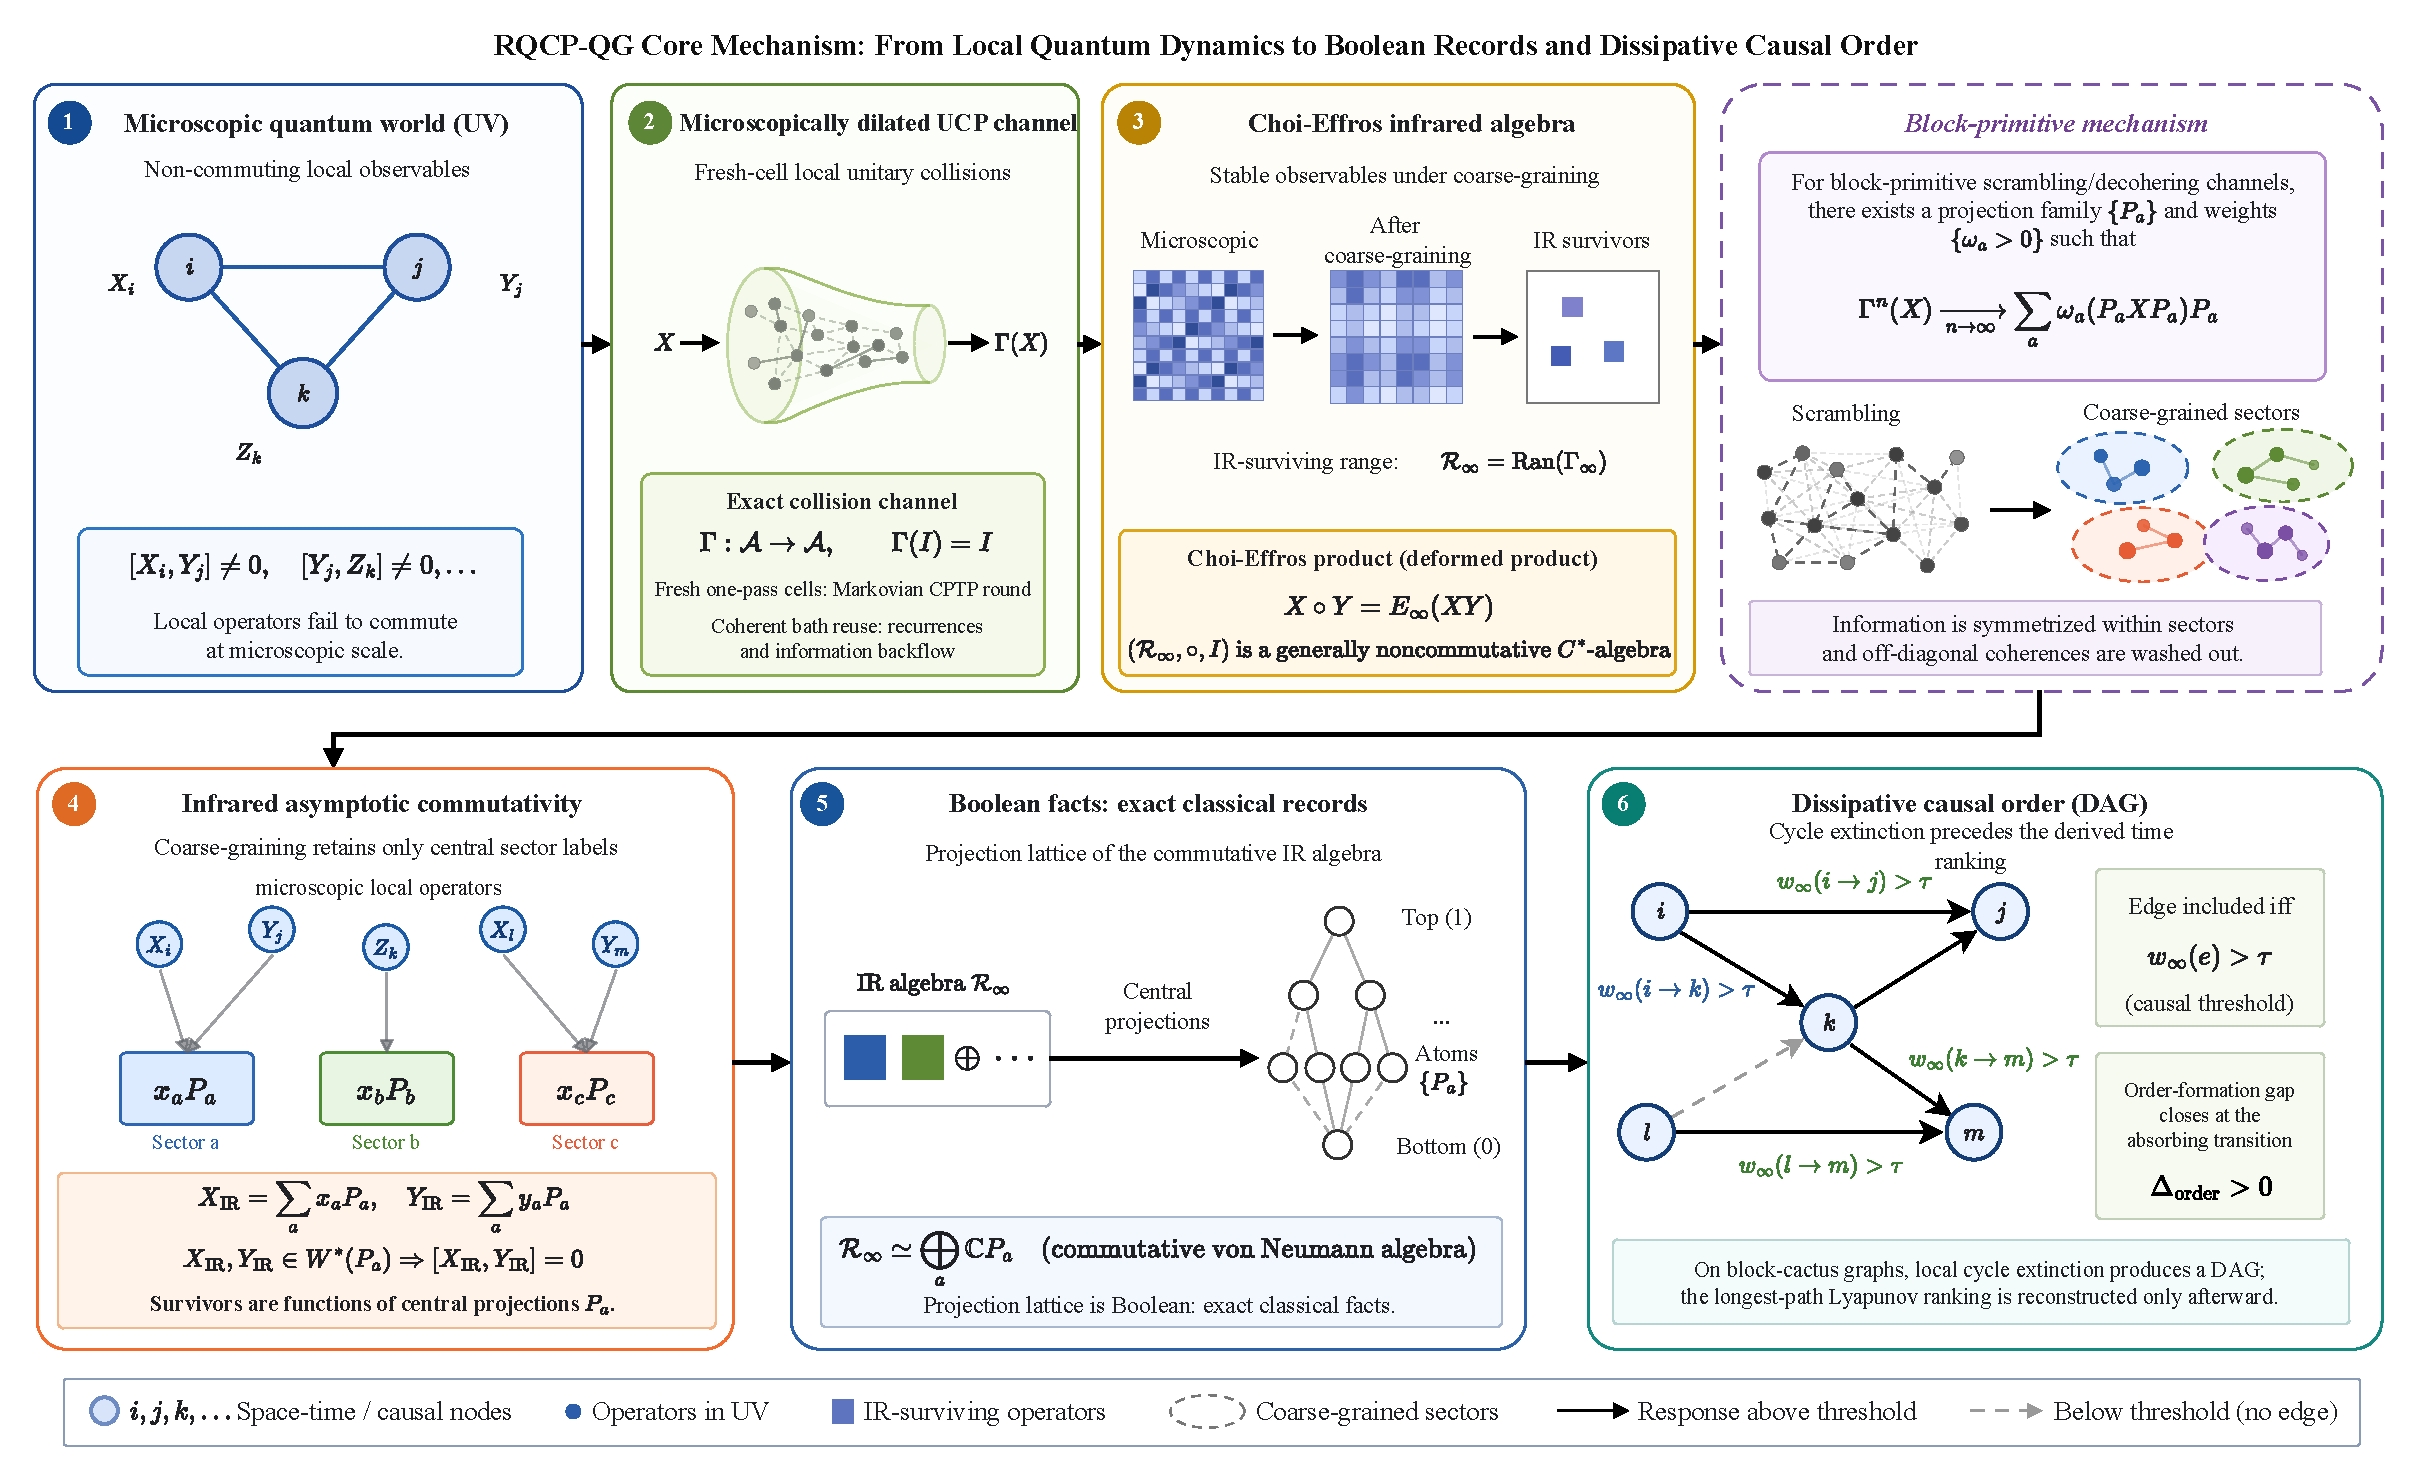
\includegraphics[width=0.96\linewidth]{figures/rqcp_qg_core_mechanism_v12.pdf}
 \caption{\textbf{The information-to-order core of RQCP-QG.}
 Panels 1--5 retain the mechanism of the original full-process diagram:
 local UCP coarse graining, a generally noncommutative Choi--Effros range,
 and its reduction to Boolean center records in block-primitive dynamics.
 The collision panel displays the fresh-cell unitary dilation realized
 by the solvable microscopic model.  Panel 6 incorporates the later
 causal-order result: local cycle defects on a block cactus become extinct
 before a DAG and longest-path Lyapunov rank are defined.  Metric geometry
 and gravity are not conclusions of this figure.}
 \label{fig:rqcp-core-mechanism}
\end{figure}
\end{landscape}

\begin{landscape}
\begin{figure}[p]
 \centering
 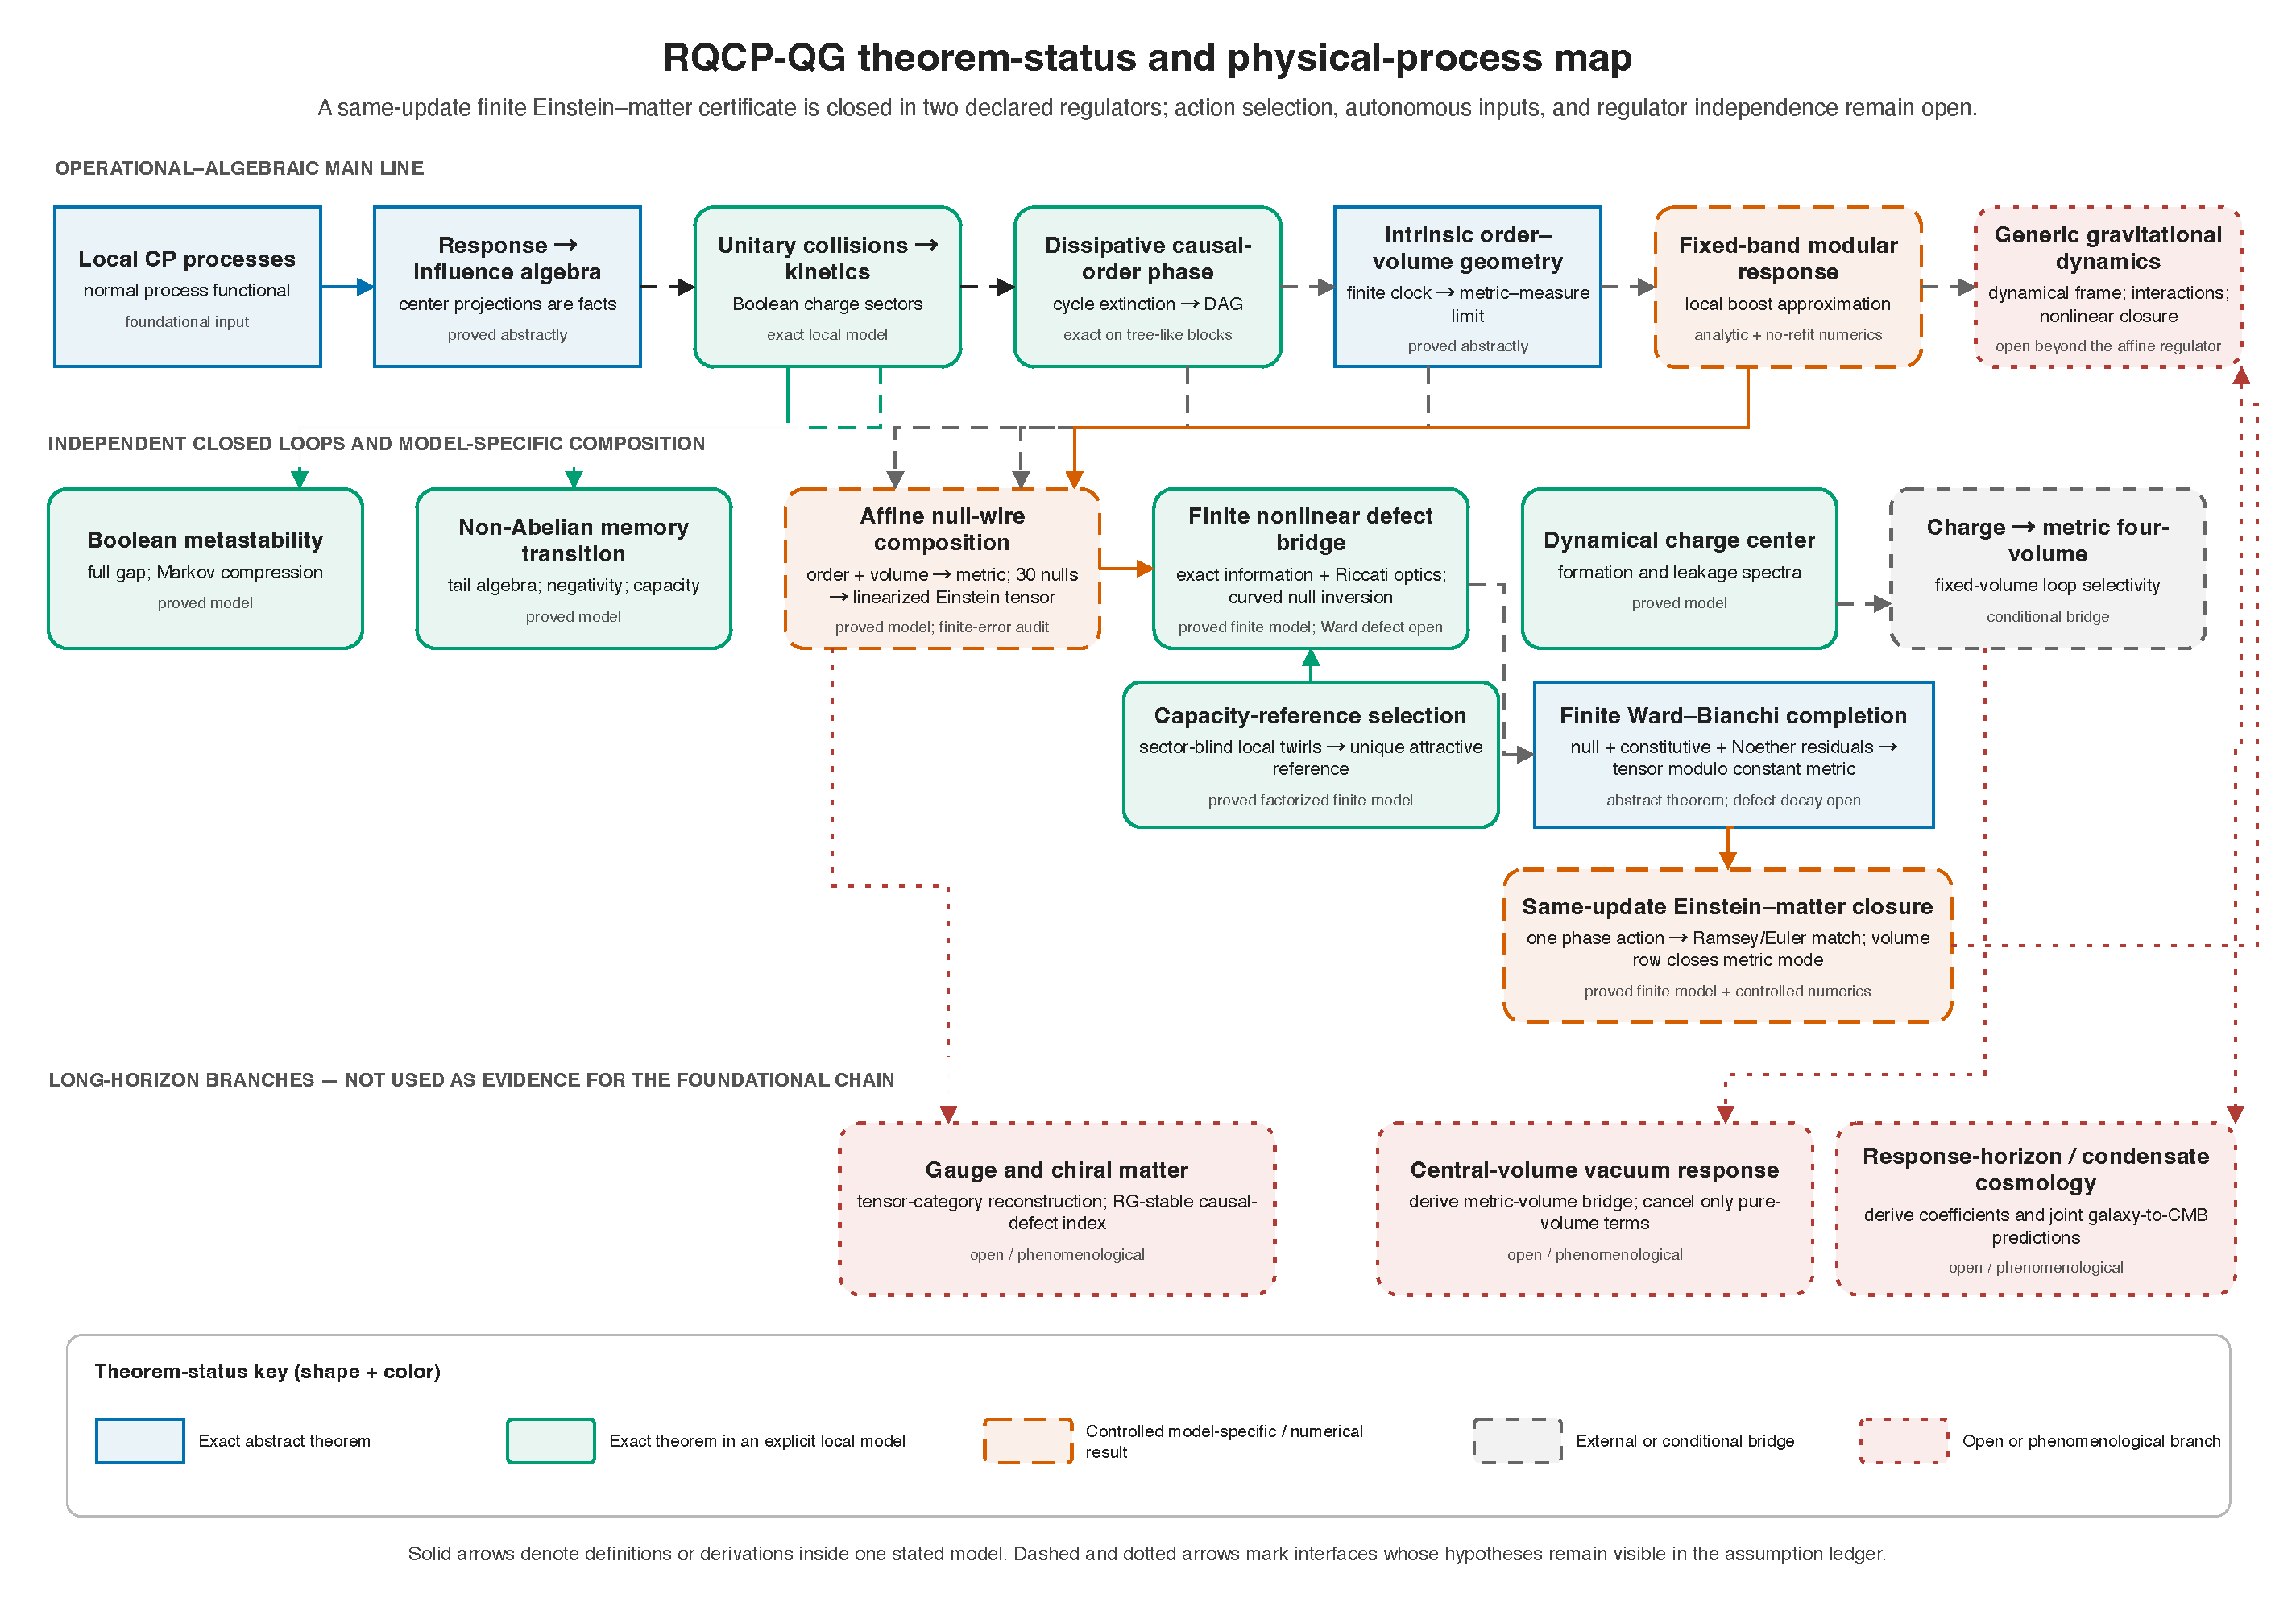
\includegraphics[width=0.819\linewidth]
 {figures/rqcp_qg_theorem_status_map_v10.pdf}
 \caption{\textbf{RQCP-QG physical processes and theorem status.}
 Blue/green denote exact abstract/model theorems; orange, gray, and red denote
 controlled, conditional, and open statements.  The lower nodes concern
 reference selection, a nonlinear Ward-defect identity, finite tensor
 completion, and a same-update Einstein--matter certificate under their
 displayed inputs.  Common refinement, relational time, quadratic
 constraints, regulator universality, and positive-Hilbert constructions are
 stated in Table~\ref{tab:status-ledger} and in their dedicated sections.  The
 common-refinement mechanism appears separately in
 Fig.~\ref{fig:unified-continuum-mechanism}.  Dashed edges are open; arrows
 between named models record logical dependence and do not identify their
 microscopic generators.}
 \label{fig:rqcp-status-map}
\end{figure}
\end{landscape}

\begin{landscape}
\subsection{Status of the principal results}

Table~\ref{tab:status-ledger} summarizes the strongest statement available
for each module and the assumptions that remain.  Any claim that an input has
been removed is restricted to the scope stated in the third column.

\footnotesize
\begin{longtable}{@{}P{0.16\linewidth}P{0.13\linewidth}
 P{0.36\linewidth}P{0.27\linewidth}@{}}
\caption{Status of the main RQCP-QG modules.}
\label{tab:status-ledger}\\
\toprule
Module & Status & Strongest present result & Remaining boundary\\
\midrule
\endfirsthead
\toprule
Module & Status & Strongest present result & Remaining boundary\\
\midrule
\endhead
Influence algebra and exact facts
& \textcolor{statusblue}{\textsf{abstract}}
& Predual response differences generate an influence algebra; its center
  projections form a complete Boolean event algebra.
& The background strategy class and field-theoretic localization remain part
  of the event context.\\
\addlinespace
Microscopic response kinetics
& \textcolor{statusgreen}{\textsf{exact model}}
& A fresh-cell unitary collision circuit gives the exact random-unitary
  channel, Boolean finite-step fixed algebra, closed Pauli hierarchy, and a
  fixed-order kinetic error independent of total system size.
& One-pass product bath cells, calibrated collision strength, and an external
  schedule remain assumptions.\\
\addlinespace
Boolean formation and metastability
& \textcolor{statusgreen}{\textsf{exact model}}
& Local dephasing and exchange give the exact charge algebra, complete
  graph-controlled gap, metastable Markov compression, topology-dependent
  tolerance, and a noncommuting leakage correction.
& The strongest norm is normalized Hilbert--Schmidt; a general
  size-independent local operator-norm theorem remains open.\\
\addlinespace
Non-Abelian memory transition
& \textcolor{statusgreen}{\textsf{exact model}}
& An occupation-time identity classifies the late-write tail algebra and
  determines reference negativity and memoryless-use quantum capacity.
& The activity quotient is classical; finite systems ultimately absorb, and
  background dephasing rounds the infinite-time phase.\\
\addlinespace
Dissipative causal order
& \textcolor{statusgreen}{\textsf{exact model}}
& Local cycle projectors on a block cactus have an exact contact-process
  quotient.  Their extinction produces a DAG and only then a longest-path
  Lyapunov ranking.
& The undirected skeleton, laboratory runtime, and extension to generic
  graphs are not generated.\\
\addlinespace
Quantum-field inverse geometry
& \textcolor{statusorange}{\textsf{model/numerical}}
& A Ramsey ratio isolates a physical covariance; six anchors fix a de Sitter
  radius, while rank-five completion predicts held-out invariants with
  perturbation and shot-noise bounds.
& Field species, state, canonical normalization, spacelike support, and the
  de Sitter model class are inputs.\\
\addlinespace
Fixed-band modular response
& \textcolor{statusorange}{\textsf{model/numerical}}
& A state-independent physical band gives an optimal finite-size response
  certificate; a sparse range-three correction passes a frozen no-refit
  holdout in the free-fermion model.
& Interactions, higher dimensions, transverse area, multiple null directions,
  and gravity are absent.\\
\addlinespace
Capacity-reference selection
& \textcolor{statusgreen}{\textsf{exact finite model}}
& Sector-blind local product-Weyl collisions select the unique
  capacity-balanced boundary reference with a size-independent
  relative-entropy contraction and an additive-block modular coefficient.
& Boundary/complement token factorization, unbiased exchange,
  \(\widehat A=a_0^2\widehat N\), correlated-record selection, and the
  continuum Newton coefficient remain inputs or open.\\
\addlinespace
Dynamical charge center
& \textcolor{statusgreen}{\textsf{exact model}}
& A local number-conserving channel isolates the complete additive-charge
  center with a graph-dependent formation gap; homogeneous breaking gives an
  exact Ehrenfest spectrum and autocorrelation.
& The microscopic \(U(1)\) law is assumed, and charge has not been proved to
  converge to metric four-volume.\\
\addlinespace
Order--volume geometry
& \textcolor{statusblue}{\textsf{abstract + conditional smooth limit}}
& A robust response DAG and positive additive record measure define an
  intrinsic finite volume clock with an exact reverse triangle.  Strong-
  profile compactness gives a Lorentzian metric--measure limit; local
  subdivision recovers proper time, dimension, measure, and good-cover
  topology for an admissible unknown smooth limit.
& Generic dynamics must still generate adjacency and acyclicity and derive a
  scale-stable capacity-density conversion.  Smoothness is certified, not
  automatic, and one absolute volume unit remains microscopic.\\
\addlinespace
Affine order--volume realization
& \textcolor{statusorange}{\textsf{model-specific}}
& On a contractible affine four-complex, Hodge loss forms an exact response
  order, Boolean record capacity gives an additive volume, and a rank-nine
  finite response frame reconstructs a Lorentzian metric with a stability
  bound.
& The affine adjacency, dimension, and 30-class null frame are inputs; this
  regulator is a composition example, not the generic compactness theorem.\\
\addlinespace
Einstein closure
& \textcolor{statusorange}{\textsf{linearized model}}
& A transverse fixed-band wire bundle, boundary record entropy, capacity
  exchange with an explicit product-reference condition, discrete focusing,
  30 null probes, conservation, and an exact lattice Bianchi identity close to
  a linearized tensor equation.
& The wires are decoupled, transverse area is calibrated,
  \(G_{\rm eff}\) is regulator dependent, and interacting modular
  universality, nonlinear focusing, and graviton self-interaction remain
  open.\\
\addlinespace
Finite nonlinear information--focusing bridge
& \textcolor{statusgreen}{\textsf{exact finite model}}
& A capacity-balanced record reference fixes the modular area coefficient;
  unitary record--bulk exchange has an exact finite relative-entropy
  remainder; a matrix Jacobi recurrence gives exact nonlinear focusing and
  area transport before caustics; and arbitrary invertible coframes preserve
  rank-nine null-tensor identifiability.
& The reference is selected only in the separate factorized token model;
  coupling it to the same nonlinear update, interacting modular response,
  shrinking-diamond locality, the nonlinear information--geometry Ward
  identity, common stress/holonomy evolution, caustics, and regulator
  independence remain open.\\
\addlinespace
Finite Ward--Bianchi tensor completion
& \textcolor{statusblue}{\textsf{abstract + finite certificate}}
& A rank-nine local null frame, compatible discrete divergence, exact
  Noether-defect chain rule, and scalar Poincar\'e gap give a noisy
  full-tensor bound modulo one constant metric mode.  Exact counterexamples
  show that null data and divergence conservation are individually
  insufficient.
& The response tensor must still be derived as the geometric Euler covector
  of the same microscopic update.  Exact holonomy Bianchi identities do not
  imply exact finite diffeomorphism symmetry, and uniform interacting
  continuum control remains open.\\
\addlinespace
Same-update Einstein--matter closure
& \textcolor{statusorange}{\textsf{proved finite model}}
& For one declared local action-phase update, a fresh Ramsey instrument and
  an independent analytic variation have controlled field and divergence
  constitutive defects.  Rank-nine null data, the finite Noether identity,
  a scalar gap, matter residuals, and one volume score then bound the complete
  geometric Euler covector, including the constant metric mode.
& The Einstein--matter action, four-dimensional regulator, signature,
  adjacency, fresh phase access, and refinement family remain inputs.
  Interacting modular dynamics, uniform general-regulator convergence, and
  a universal Newton coefficient are not derived.\\
\addlinespace
Unified operational continuum limit
& \textcolor{statusorange}{\textsf{proved model + interface theorem}}
& One common \(h\) and one register family generate the response order,
  integer record capacities, and the phase action.  A joint discrepancy
  controls Lorentzian metric--measure convergence and the weak
  Einstein--matter Euler limit on the geometry reconstructed from those same
  records.  FLRW and four-dimensional TT refinements pass independent split
  controls.
& The four-dimensional topology, Einstein--Hilbert--scalar action, capacity
  unit, and \(G_h=G\) are supplied.  General nonlinear inhomogeneous
  convergence, autonomous phase/action selection, quantum fluctuations, and
  renormalization remain open.\\
\addlinespace
Same-link induced quantum TT gravity
& \textcolor{statusgreen}{\textsf{proved model}}
& A compiled anonymous pair constructor produces an unlabeled
  \(P_L\times T_L^3\) record lattice.  Its active links supply directed order,
  integer record volume, and scalar hopping.  With no bare curvature action,
  the scalar determinant has a strictly positive TT two-derivative
  coefficient; the saddle-selected, rescaled fixed-band TT Schwinger
  functions have a controlled Gaussian large-\(N_s\) limit.  One joint discrepancy controls
  constructor, order--volume, determinant, and quantum errors.
& The four-dimensional graph language, program/clock state, fair scheduler,
  one-cell volume unit, scalar species, fixed spacing, and a local \(q=0\)
  TT saddle measure are inputs.  The result is fixed-volume and plus-polarized, leading order
  at large \(N_s\), and has no graph backreaction, cutoff removal, universal
  \(G\), or nonlinear gauge-complete graviton measure.\\
\addlinespace
Finite relational order--volume history
& \textcolor{statusgreen}{\textsf{proved model}}
& A stationary local propagation Hamiltonian has an exact conditional
  Page--Wootters history.  Legal rank-increasing append records give a
  schedule-independent DAG, and the same accepted records carry an additive,
  blocking-stable information volume with \(O(L^{-2})\) weak convergence.
& The low-entropy clock endpoint, update program, parent-port law,
  four-dimensional branch, and microscopic volume unit are inputs.  The
  result is finite and does not select an eternal clock or generic
  Hamiltonian basin.\\
\addlinespace
Quadratic Einstein constraint completion
& \textcolor{statusgreen}{\textsf{proved model}}
& The induced TT normalization uniquely fixes the ten-component
  Fierz--Pauli kernel.  One common lattice derivative gives four exact gauge
  zero modes, de Donder ghosts, a nilpotent linear BRST differential,
  gauge-independent conserved-source response, and a full fixed-band
  continuum limit.
& Linear gauge symmetry and the conformal contour are model contracts.
  Nonlinear constraints, cubic Slavnov--Taylor identities, the BV master
  equation, and a nonperturbative metric measure remain open.\\
\addlinespace
Regulator-independent Newton flow
& \textcolor{statusblue}{\textsf{proved regulator-class theorem}}
& Positive determinant weights are obstructed from a cutoff-free Newton
  limit.  Vanishing zeroth and mass-squared supertrace moments remove the
  power, logarithmic, and scheme-local terms; three inequivalent regulators
  converge to one positive logarithmic mass invariant and fixed physical
  Gaussian band.
& The signed supertrace is an input to this regulator theorem.  BRIDGE-PH1
  derives it in a separate free positive-Hilbert model.  The absolute value
  is spectrum dependent, and vacuum plus higher-curvature moments are not
  balanced.\\
\addlinespace
Positive-Hilbert spectral balance
& \textcolor{statusgreen}{\textsf{proved model}}
& Exterior parity on \(\Lambda^\bullet\mathbb C^2\) and an additive
  number-operator mass ladder derive \((1,-2,1)\),
  \(\Str\mathbf1=\Str M^2=0\), a positive finite logarithmic invariant,
  transfer-form positivity, geometry-by-geometry persistence under any
  supplied finite positive graph sum, and exact finite-move response.
& The construction is free; its graph support and prior are supplied.
  Exact all-level pairing is proved to erase the finite invariant, while
  generic interactions break the balance.  Finite interacting protection,
  projective positive growth, and a covariant rank-one coherent branch are
  supplied separately below; a Lorentzian continuum, spin--statistics, and
  nonlinear gravity are not derived.\\
\addlinespace
Selective Ward, projective, covariant, and non-Abelian histories
& \textcolor{statusgreen}{\textsf{proved models}}
& A shifted CAR Ward identity protects the positive response for arbitrary
  finite interacting physical operators.  Conditional causal births extend
  it to exact deletion-projective cylinder laws, an infinite past-finite
  labelled-history measure, CPTP channels, and path-response identities.  A
  contact-response CSG subfamily additionally has exact discrete general
  covariance and Bell causality; a one-arity \(r\ge2\) complex branch extends
  to a countably additive measure and a strongly positive rank-one
  decoherence functional with nonzero finite-volume interference.  On a
  separate fixed two-port strip, fresh-ancilla noncommuting decisions give
  an extendible rank-four strongly positive history measure.  On arbitrary
  CSG causal histories, intrinsic fresh-event Pauli holonomies define a
  covariant countably additive non-Abelian operator measure and strongly
  positive grade-2 decoherence functional; a late-cylinder bound proves that
  integration does not abelianize its range.
& The commutant, maximal-birth language, contact motifs, response multiplet,
  parameters, coherent arity, phase, and two-port strip are supplied.  The
  arbitrary-causet non-Abelian construction uses a classical CSG density:
  it does not satisfy an operator Markov sum or square-operator
  TOBC/NTOBC/CPOBC, and has no quantum geometry backreaction.  No tight
  Lorentzian continuum or nonlinear constraint dynamics is derived.\\
\addlinespace
Central operator-valued causal growth
& \textcolor{statusgreen}{\textsf{proved model + classification}}
& Positive central CSG couplings give exact parentwise POVMs, covariant
  L\"uders path effects, central Bell cross-products, and a strongly
  countably additive infinite-history POVM.  Every such law is a direct
  integral of scalar CSG laws, so geometry statistics are blind to
  coupling-sector coherence.  A positive noncentral normalized control
  fails DGC.
& The central branch is state controlled but not coherent quantum
  backreaction.  No noncentral covariant operator Bell/Markov law,
  discarded-record infinite instrument, tight Lorentzian continuum, or
  nonlinear constraint closure is derived.\\
\addlinespace
Bell-causal operator-growth rigidity
& \textcolor{statusgreen}{\textsf{exact boundary theorem}}
& Every finite-dimensional self-adjoint nonsingular CPOBC transition
  system is commutative without a sign assumption, including
  complementary-spectrum blocks.  At the
  \(t=1/4\) scalar CSG point, exact four-event deformation theory
  independently forces all leading matrix tangents to commute; every
  \(2\times2\) upper-triangular extension between distinct strictly
  positive scalar CSG coupling sequences is split, at arbitrary
  first-difference order, while every coincident-character
  \(2\times2\) self-extension is a commuting coupling tangent.  An
  irreducible nonsingular \(2\times2\) branch with non-scalar
  \(R_2=Q_1^{-1}Q_2\) is excluded by exact next-stage minors.  On the
  remaining scalar branch, the two-chain condition excludes \(h=1\).
  Within the trace-balanced subchart \(d=a,\ x=-1\) of the normalized
  first-simple-spectrum chart at \(R_3\), exact factorization leaves three
  components, all excluded at the next antichain stage.
& Non-self-adjoint nonsingular and singular transitions, state-only
  covariance, higher-dimensional noncommutative nilpotent thickenings,
  the remainder of the normalized first-simple-spectrum chart,
  delayed-onset irreducible nontriangular representations with scalar
  \(R_2=h\mathbf1\), \(h\ne0,1\), and Jordan/later onset,
  and a projectively consistent infinite noncommutative CPOBC measure remain
  open.  The result is a self-adjoint nonsingular no-go theorem, not a
  construction or a no-go theorem for every operator-history formulation.\\
\addlinespace
Autonomous geometry and gravity
& \textcolor{statusred}{\textsf{open}}
& The intrinsic bridge supplies finite geometry and a generic
  metric--measure endpoint.  Three additional model chains supply a
  finite relational clock, quadratic BRST completion, and a
  regulator-independent balanced Newton limit.
& One autonomous background-free dynamics must still select adjacency,
  dimension, and the capacity-density law; protect the balanced multiplet
  under interacting Lorentzian RG; and produce nonlinear gravitational
  dynamics and the quantum metric measure.\\
\addlinespace
Vacuum, matter, and cosmology
& \textcolor{statusgray}{\textsf{conditional}}
& Fixed-sector normalization cancels a pure-volume term; standard tensor
  category, index, and effective-field-theory constructions identify precise
  targets.
& The central-volume bridge, gauge-category attractor, chiral-index selection,
  response-horizon coefficients, and dark equation of state are not derived.\\
\bottomrule
\end{longtable}
\end{landscape}

\subsection{Relation to the companion manuscripts}

The completed finite-model results are maintained as independent manuscripts.
Table~\ref{tab:companion-correspondence} fixes their current titles and
roles.  The labels PRL-1--PRL-5 are internal indices, not serial titles or
logical implications between adjacent entries.  The Boolean/metastability
Letter is denoted PRL-0 because it supplies the finite-system reference model
for the collision, memory, and central-charge studies.

\begin{longtable}{@{}P{0.10\textwidth}P{0.37\textwidth}P{0.45\textwidth}@{}}
\caption{Relation between the outstanding assumptions and the companion
manuscripts.  Each manuscript contains an independent
theorem--model--observable result; open compositions are stated separately
in Sec.~\ref{sec:updated-core-boundary}.}
\label{tab:companion-correspondence}\\
\toprule
Index & Canonical title & Unique role in the program\\
\midrule
\endfirsthead
\toprule
Index & Canonical title & Unique role in the program\\
\midrule
\endhead
\midrule
\multicolumn{3}{r}{\small Continued on the next page}\\
\endfoot
\bottomrule
\endlastfoot
PRA & \emph{Microscopic Derivation of Quantum Response Kinetics from Local
Unitary Dynamics}
& Derives the dephasing--random-SWAP kinetics, fixed-response hierarchy, and
finite-step error from fresh one-pass unitary collisions.\\
PRL-0 & \emph{Metastable Classical Dynamics of Noise-Selected Charge Sectors}
& Solves the exact Boolean algebra, full gap, weak-perturbation reduction, and
topology-dependent tolerance of that kinetic generator.\\
PRL-1 & \emph{Causal Order as a Dissipative Phase of Local Quantum Channels}
& Generates DAG order from cycle-defect extinction on a block cactus, without
supplying a Lyapunov function in advance.\\
PRL-2 & \emph{Dynamical Transition between Classical Records and Non-Abelian
Quantum Memory}
& Gives an exact late-write tail-algebra and quantum-capacity transition under
an absorbing noise field.\\
PRL-3 & \emph{Lorentzian Curvature from Sparse Quantum-Field Correlations}
& Infers an unknown de Sitter scale and blind invariants inside a prescribed
field--state--geometry family.\\
PRL-4 & \emph{Fixed-Band Modular-to-Boost Response in a Critical Quantum
Lattice}
& Replaces a shrinking fixed-mode window by a state-independent fixed physical
band and a finite-cutoff response certificate.\\
PRL-5 & \emph{Dynamical Formation and Controlled Decay of Charge
Superselection}
& Derives the complete charge center, sectorwise CPTP restrictions, exact
lumpability, and controlled breaking, while leaving charge-to-volume open.\\
BRIDGE-OV1 & \emph{An Intrinsic Order--Volume Bridge from Quantum Response to
Lorentzian Metric--Measure Geometry}
& Constructs the finite volume clock and generic Lorentzian metric--measure
limit, proves the continuum proper-time identity and smooth-limit error
budget, and turns nonmanifold behavior into explicit rejection certificates;
it consumes rather than dynamically generates the input order and
capacity-density law.\\
BRIDGE-1 & \emph{Order--Volume Reconstruction and Linearized Einstein Closure
in a Quantum Null-Wire Lattice}
& Closes the order--volume and multi-null Einstein interfaces in one affine,
decoupled-wire regulator, with an exact rank certificate and finite-error
ledger; it leaves generic and nonlinear completion open.\\
BRIDGE-NL1 & \emph{Finite Quantum-Information Remainders and Nonlinear Null
Focusing in a Quantum Record Lattice}
& Replaces the finite-exchange entropy first law and linearized optical law by
exact identities, proves curved rank-nine null inversion, and isolates the
remaining nonlinear Einstein content as a measurable Ward-defect condition.\\
BRIDGE-REF1 & \emph{Local Unitary Selection of a Capacity-Balanced Area
Reference}
& Selects the capacity-balanced reference in a factorized
capacity--complement token model, proves a size-independent entropy
contraction and bias test, and preserves the modular coefficient under
additive blocking.\\
BRIDGE-WB1 & \emph{Quantitative Ward--Bianchi Completion on Finite
Lorentzian Record Lattices}
& Converts local null, symmetry, matter-equation, and measurement residuals
into a certified full-tensor estimate, while exposing the still-open
constitutive identification with the geometric Euler derivative.\\
BRIDGE-SU1 & \emph{Same-Update Quantum Response and Einstein--Matter Ward
Closure on Finite Lattices}
& Derives the field and divergence constitutive budgets from one declared
local action-phase process through independent Ramsey and analytic pipelines;
one volume score fixes the missing constant metric mode.  This is a finite
model theorem, not dynamical selection of the action or a universal
continuum limit.\\
BRIDGE-UC1 & \emph{A Unified Operational Continuum Limit for Lorentzian
Geometry and Einstein Response}
& Uses one register family and one refinement parameter for the
order--volume and action-phase branches, proves a joint
metric--measure/Einstein--Euler limit, and rejects split geometry or split
action by a nonzero finite discrepancy.  Its explicit FLRW--TT realization
is model-specific and supplies rather than selects the gravitational action,
dimension, capacity unit, and Newton coefficient.\\
BRIDGE-IQ1 & \emph{From Relational Order--Volume Records to Induced Quantum
Gravity on the Same Links}
& Replaces the prescribed Einstein--Hilbert phase of BRIDGE-UC1 by a
strictly positive two-derivative TT kernel induced by linked scalar matter
on the constructor output, and gives a fixed-band large-\(N_s\) quantum
limit for that same kernel.  It compiles rather than selects dimension,
topology, clock, volume unit, and matter content, and it does not construct
the gauge-complete nonlinear theory or a regulator-independent Newton flow.\\
BRIDGE-AT1 & \emph{Relational Time and Autonomous Order--Volume Growth in a
Closed Quantum Network}
& Replaces the external update parameter by an exact finite stationary
history sector and proves that conditional rank-increasing growth, causal
incidence, capacity, and weak volume share one record refinement.  The
clock/program boundary and four-dimensional port language remain inputs.\\
BRIDGE-QC1 & \emph{Constraint-Complete Quantum Einstein Response from an
Induced Transverse--Traceless Coefficient}
& Extends the induced TT coefficient uniquely to the ten-component
Fierz--Pauli kernel and closes its finite lattice Ward, ghost, BRST, and
conserved-source Gaussian response at quadratic order.\\
BRIDGE-RG1 & \emph{Spectral Balance and a Regulator-Independent Induced
Newton Coupling}
& Proves the positive-spectrum obstruction, the necessity and sufficiency
of two spectral moments, and a common fixed-band limit across sharp
momentum, sharp proper-time, and smooth proper-time schemes; the signed
balance itself remains microscopic input.\\
BRIDGE-PH1 & \emph{A Positive-Hilbert Origin for Spectral Balance in
Induced Gravity}
& Derives the balanced weights and masses from exterior parity and an
additive internal number operator on a positive Fock space, proves
geometry-by-geometry persistence in any supplied finite graph ensemble and
exact finite-move response, and exposes both the nonlinear-mass defect and
the exact-pairing obstruction.\\
BRIDGE-SLW1 & \emph{Selective Ladder Ward Protection and Positive Dynamics
of Finite Quantum Geometries}
& Characterizes the exact shifted-CAR Ward manifold for an arbitrary finite
positive interacting physical operator, bounds approximate Ward and heat
defects, and realizes the surviving positive response as the unique
stationary law of a local unitary-dilatable finite-geometry channel.  The
internal commutant and finite geometry language remain supplied, and no
projective continuum measure or nonlinear gauge closure is claimed.\\
BRIDGE-PCG1 & \emph{Projectively Consistent Quantum-Response Growth of
Causal Histories}
& Extends the protected positive response to conditionally normalized
causal births, exact deletion-projective cylinder laws, a probability
measure on infinite past-finite labelled histories, and exact path-response
identities.  Natural labels and the growth language remain supplied; no
discrete general covariance, coherent quantum measure, or Lorentzian
continuum limit is claimed.\\
BRIDGE-CQG1 & \emph{Covariant Quantum-Response Growth and an Extendible
Quantum Measure on Causal Histories}
& Converts response-generated contact-star weights into a nonvanishing
classical sequential-growth law with exact deletion projectivity, discrete
general covariance, and Bell causality.  A separate one-arity \(r\ge2\)
complex response has bounded variation, a unique countably additive
extension, a normalized strongly positive rank-one decoherence functional,
and nonzero finite-volume quotient interference.  The growth language,
contact family, arity, and phase remain supplied; no local-unitary
non-rank-one history dynamics or Lorentzian continuum limit is claimed.\\
\addlinespace
BRIDGE-NQH1 & \emph{Extendible Non-Abelian Quantum History Measures from
Local Unitary Decisions}
& On a fixed ranked two-port causal strip, two fresh-ancilla decisions obey
exact operator Markov and Kraus identities, generate a noncommuting
transition algebra, and have a countably additive matrix-measure extension
whenever the response-angle tail is summable.  The induced decoherence
functional is strongly positive, has nonzero interference, and reaches the
full rank-four Hilbert--Schmidt bond space after two cells.  The port
language and foliation remain supplied, and this theorem does not solve
unlabeled operator Bell causality on arbitrary causal sets or a Lorentzian
continuum limit.\\
\addlinespace
BRIDGE-CNH1 & \emph{Covariant Non-Abelian Quantum Measures from
Spectator-Local Causal Holonomies}
& On arbitrary response-generated CSG histories, each birth rotates only a
fresh event qubit by an intrinsic precursor-dependent Pauli gate.  An
exponential seed-tail theorem gives an operator-norm infinite product, a
countably additive bounded-variation \(B(\mathcal H)\)-valued measure, and
a normalized strongly positive grade-2 decoherence functional.  Exact
relabeling equivariance, spectator invariance, and a late-cylinder lower
bound prove a noncommuting integrated range.  The scalar CSG law remains
external to the operator density; this is isometric Bell locality, not a
square-operator CPOBC solution, and no continuum or constraint theorem is
claimed.\\
\addlinespace
BRIDGE-OCG1 & \emph{Central Operator-Valued Causal-Set Growth and the
Boundary of Coherent Backreaction}
& Solves the commutative operator-valued CSG branch: central positive
couplings give exact finite POVMs, DGC, Bell cross-products, and an infinite
history POVM, but a direct-integral theorem proves coherence blindness of
the geometry marginal.  A positive noncentral normalized control violates
DGC, and an independent fresh-event instrument shows that non-Abelian
records can coexist without geometry backreaction.\\
\addlinespace
BRIDGE-BCGR1 & \emph{Self-Adjoint and All-Order Triangular Rigidity in
Bell-Causal Quantum Sequential Growth}
& Attacks the remaining nonsingular square-operator CPOBC equations rather
than adding a separate noncommuting density.  It proves commutativity of
every finite-dimensional self-adjoint nonsingular CPOBC system without a
sign assumption, an exact rank obstruction to every noncommuting leading
tangent at the four-event \(t=1/4\) scalar point, and an all-order
determinant proving splitting of every \(2\times2\) upper-triangular
extension between distinct strictly positive scalar CSG coupling
sequences and classifies every coincident-character \(2\times2\)
self-extension as a commuting dual-number coupling tangent.  It also
excludes irreducible nonsingular \(2\times2\) onset at non-scalar \(R_2\);
the two-chain condition removes the scalar value \(h=1\), and exact
certificates obstruct all three components in the trace-balanced
\(d=a,\ x=-1\) subchart of the normalized delayed first-simple-spectrum
chart at the following antichain stage.
It leaves non-self-adjoint nonsingular, zero/singular-coupling, state-only,
higher-dimensional noncommutative nilpotent, delayed-onset irreducible
nontriangular components with scalar
\(R_2=h\mathbf1\), \(h\ne0,1\), Jordan/later onset, and infinite branches
explicitly open; the remainder of the normalized first-simple-spectrum
chart is also open.\\
\end{longtable}

The original exact interface between two manuscripts is
\[
 \text{PRA collision circuit}
 \longrightarrow
 \text{PRL-0 dephasing--exchange generator}.
\]
BRIDGE-OV1 closes the mathematical composition from any certified
order--record input to a Lorentzian metric--measure output; it does not
identify the PRL-1 block-cactus dynamics with a universal capacity-density
law.  BRIDGE-1 is not a relabeling of PRL-1+PRL-3.  It introduces an affine
regulator whose Hodge order, Boolean volume, finite null frame, transverse
modular response, and lattice focusing are proved to compose internally.  It
reuses the fixed-band certificate of PRL-4 but does not identify the PRL-1
block-cactus generator with the PRL-3 de Sitter detector model.  The general
autonomous order--capacity generation, autonomous Einstein-phase selection,
and the BRIDGE-OV1+PRL-5 central-volume limit remain open.  BRIDGE-REF1 closes
reference selection only for factorized tokens and is not identified with
the nonlinear record--geometry generator of BRIDGE-NL1.  BRIDGE-WB1 closes
only the finite tensor-completion step.  BRIDGE-SU1 supplies the missing
same-update response--Euler theorem and constant-mode volume row in two
declared regulators; it does not derive their Einstein--matter phase action,
geometry, or universal continuum limit from the preceding record dynamics.
BRIDGE-UC1 then closes the compatibility of the order--volume and
same-update limits for one common FLRW--TT refinement family.  It proves that
the two continuum outputs refer to the same records and metric, while leaving
autonomous selection of that refinement family and action open.
BRIDGE-IQ1 closes a different missing interface: on one compiled anonymous
record lattice it removes the bare Einstein--Hilbert phase and derives a
positive TT kinetic coefficient from scalar matter carried by the same
links.  Its large-\(N_s\) limit quantizes only that fixed-volume infrared
sector.  It neither upgrades the compiled language to the generic
background-free target of BRIDGE-OV1 nor supplies the nonlinear tensor
completion demanded by P9.
BRIDGE-AT1 replaces its external scheduler by a finite relational history
and makes causal rank and information volume records of that same history.
BRIDGE-QC1 then closes the full quadratic gauge complex normalized by the
induced TT response.  BRIDGE-RG1 removes the cutoff only after a signed
two-moment balance is imposed.  BRIDGE-PH1 derives that balance from a
positive free graph multiplet.  BRIDGE-SLW1 supplies exact and approximate
selective protection for an arbitrary finite positive interacting physical
operator and a positive local dynamics for the induced weights on a supplied
finite geometry language.  BRIDGE-PCG1 then removes the independent
finite-size normalization defect by constructing exactly projective laws and
an infinite positive measure on a supplied naturally labelled causal-birth
language.  BRIDGE-CQG1 then removes the natural-label path-weight and
Bell-spectator defects for a response-generated contact CSG subfamily and
constructs an extendible rank-one coherent quantum measure with nonzero
finite-volume interference.  BRIDGE-NQH1 separately removes the rank-one
and local-realizability restrictions on a fixed two-port strip.
BRIDGE-CNH1 then combines arbitrary-down-set CSG covariance with intrinsic
fresh-event noncommuting holonomies and a countably additive operator-valued
measure.  It does not solve the square-operator Bell equations or make the
geometry probability law quantum and backreacting.  BRIDGE-OCG1 then closes
and classifies the central operator-valued branch: its infinite POVM is
exactly covariant, but is only a direct integral of scalar laws, while a
positive noncentral normalized control fails DGC.  It therefore rules out
centralization as the missing coherent-backreaction mechanism rather than
closing that mechanism.  BRIDGE-BCGR1 then proves that three natural
noncentral escape routes are rigid: every finite-dimensional self-adjoint
nonsingular system commutes without a sign assumption, noncommuting leading
tangents at the tested scalar point are obstructed, and the complete
distinct positive scalar CSG \(2\times2\) triangular family splits at
arbitrary first-difference order; the coincident-character branch consists
only of commuting coupling tangents, and irreducible nonsingular
\(2\times2\) onset at non-scalar \(R_2\) is impossible.  It does not
exclude a non-self-adjoint nonsingular, zero/singular-coupling, state-only,
higher-dimensional noncommutative nilpotent, or the remaining delayed-onset
irreducible nontriangular representations with scalar
\(R_2=h\mathbf1\), \(h\ne0,1\), including Jordan or later onset, and it
does not provide
an infinite extension.  These
manuscripts still do not derive the
protected internal commutant, maximal-birth/port language, contact motifs,
response multiplet, coherent arity or phase, a covariant non-Abelian history
law satisfying operator Markov/Bell constraints, a tight Lorentzian
continuum, continuum spin--statistics, or a nonlinear BV identity.  The
interfaces therefore compose at finite or quadratic
regulator level, but they are not evidence that the clock program, gauge law,
matter multiplet, growth language, or interacting continuum spectrum is
dynamically selected.

\subsection{Microscopic, kinetic, and continuum limits}

The methodological standard is close in spirit to the modern treatment of
Hilbert's sixth problem: microscopic dynamics, kinetic evolution, and
macroscopic equations are different limits, and each arrow needs its own
error estimate and order of limits.  Long-time derivations of Boltzmann
dynamics from hard spheres and subsequent fluid limits make this separation
explicit \cite{DengHaniMa2024,DengHaniMa2025}.  RQCP-QG has a different
microscopic object and does not inherit those theorems, but it should inherit
their discipline.  We therefore distinguish
\begin{equation}
 \text{local unitary process}
 \ \longrightarrow\
 \text{quantum response kinetics}
 \ \longrightarrow\
 \text{hydrodynamic or geometric field}.
 \label{eq:three-scale-standard}
\end{equation}
The first arrow asks for a microscopic dilation, a controlled memory
assumption, and a finite-time channel bound.  The second asks for the relevant
slow variables, a kinetic or spectral gap, a scaling regime, and a continuum
error.  A successful calculation at the middle level does not validate the
last arrow.  This is why the collision model below is a foundational advance
even though it does not generate a metric, and why the modular lattice result
is not called an Einstein derivation.

\subsection{Boundary of the present results}

The present results do not show that a single \emph{background-independent}
microscopic model yields
\[
\begin{gathered}
\text{quantum process}\to\text{generic curved Lorentzian spacetime}
\to\text{nonlinear Einstein dynamics}\\
\to\text{Standard Model and cosmology}.
\end{gathered}
\]
In particular:
\begin{enumerate}
\item the causal-order model generates order on a restricted graph family,
not the graph itself or a metric;
\item the inverse-geometry model infers curvature inside a specified
geometry--state class and does not establish spacetime emergence;
\item the intrinsic order--volume bridge constructs geometry only after a
robust order and positive additive record measure pass their gates; it does
not derive generic adjacency, the capacity-density conversion, or an
autonomous runtime from one closed dynamics;
\item the modular lattice model ends with a response certificate and does not
derive a gravitational field equation;
\item the affine null-wire bridge derives a linearized field equation only
after fixing the four-complex, response cone, decoupled-wire regulator, and
linear-response regime; it does not derive their generic selection or
nonlinear completion;
\item the nonlinear finite-regulator bridge derives exact information and
optical remainder identities before caustics, but not their required Ward
matching, an interacting modular limit, covariant stress/Bianchi evolution,
or a regulator-independent Einstein equation;
\item capacity-reference selection is proved only for factorized tokens.  It
does not derive the record--area map, correlated-record reference, or
observed Newton coefficient;
\item the finite Ward--Bianchi theorem controls tensor completion under a
constitutive identification; it does not derive that identification or
promote a holonomy identity into an exact finite diffeomorphism symmetry;
\item the same-update bridge derives the constitutive identification and
constant-mode score only for a prescribed local Einstein--matter phase
action; it does not derive that action, its four-dimensional regulator, or a
universal Newton normalization from the preceding record dynamics;
\item the unified-continuum bridge proves that order, volume, response, and
the Euler limit use one common FLRW--TT refinement, but it does not derive
the four-dimensional manifold phase, the Einstein--Hilbert action, the
capacity unit, \(G\), or a general quantum probability-law limit;
\item the same-link induced-gravity bridge removes the bare curvature action
only inside a compiled \(3+1\)-dimensional record language and a fixed-volume
TT sector.  It retains the program/clock, fair scheduler, volume unit,
microscopic spacing, scalar matter content, and local TT measure; its
large-\(N_s\) infrared limit is not a cutoff-free or gauge-complete quantum
gravity measure;
\item the relational-history model replaces external runtime only within a
prepared finite clock and program.  It does not select those inputs, the port
language, four dimensions, or the physical record-volume unit;
\item the constraint-complete model is gauge complete only at quadratic
order after the linear gauge law is declared; nonlinear BV/BRST closure and
a nonperturbative metric measure are absent;
\item the regulator-independent Newton theorem requires a signed
two-moment determinant balance.  The companion positive-Hilbert model
derives that balance for a free affine mass ladder on every member of a
supplied finite graph ensemble and rules out exact all-level pairing as the
sole protection.  The selective-Ward companion protects the same moments
for arbitrary finite positive interacting physical operators and samples
their positive weights on a supplied finite geometry language.  The
projective-growth companion further turns those weights into compatible
finite cylinder laws and an infinite positive history measure on a supplied
naturally labelled causal-birth language.  The covariant-growth companion
adds a response-generated contact CSG subfamily with exact discrete general
covariance and Bell causality and an extendible rank-one coherent measure.
The fixed-strip companion separately supplies a local-unitary
noncommutative rank-four measure with a countable extension.  The
arbitrary-causet holonomy companion combines the classical CSG density
with intrinsic fresh-event noncommuting gates to obtain a
relabeling-covariant countably additive operator measure whose integrated
range is provably non-Abelian.  The central operator-growth companion proves
that a commutative operator promotion has an exact infinite POVM but is
only a direct mixture of scalar laws; its positive noncentral normalized
control fails DGC.  These results do not derive the internal
commutant, maximal-birth/port language, contact motifs, response multiplet,
coherent arity, or phase.  In particular, the arbitrary-causet construction
retains an external classical CSG law and does not satisfy an operator
Markov sum or the square-operator TOBC/NTOBC/CPOBC conditions, while the
central branch is coherence blind; neither supplies a quantum-backreacting
geometry law.  The companions do not
prove Lorentzian continuum refinement,
spin--statistics or anomaly freedom, absolute Newton constant, or vacuum and
higher-curvature renormalization;
\item the charge-center model derives a superselection structure but not its
identification with metric volume;
\item the response-horizon, finite spectral triple, generation-number, and
response-superfluid sectors are research targets rather than consequences of
the foundational theorems.
\end{enumerate}
These exclusions are part of the theory's falsifiability.  They prevent an
application of a conditional synthesis theorem from being mistaken for a
microscopic derivation.
